\section{Table}

\begin{table}[htp]
    \centering
    \begin{tabular}{r|l|p{10cm}}
        Right &  Left  &  Longlonglonglonglonglonglonglong longlonglonglonglonglonglonglonglonglonglonglonglong longlonglonglonglonglong \\
        Right &  Left  &  Longlonglonglonglonglonglong
        longlonglonglonglonglonglonglong
        longlonglonglong
        longlonglonglonglonglonglonglong 
    \end{tabular}
    \caption{This is a caption}
    \label{tab:trans-sym}
\end{table}

\section{List}
This is a List:
\begin{itemize}
    \item \textbf{Bullet 1}: Bullet 1 is bullet 1.
    \item \textbf{Bullet 2}: Bullet 2 is bullet 2.
\end{itemize}

\section{Definition}
\begin{definition}\label{def:def1}
\textbf{DEFINITION NAME}: This is a definition.
\end{definition} 

\section{Tikz Pictures}
\begin{figure}[htp]
    \centering
        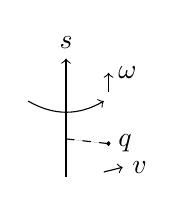
\begin{tikzpicture}[scale=0.6]
            \draw[->] (0,-1)--(0,1.5)node[above] {$s$};
            \draw[->] (-0.8,0.6) to[bend right] (0.8,0.6);
            \draw[->] (0.9, 0.8)--(0.9, 1.2) node[right] {$\omega$};
            \filldraw[dashed] (0,-0.2)--(0.9, -0.3) circle (1pt) node [right] {$q$};
            \draw[->] (0.8, -0.9)--(1.2, -0.8) node[right] {$v$};
        \end{tikzpicture}
    \caption{This is a caption. }
    \label{fig:rotation}
\end{figure}

% avoid bad break
\vspace{5cm} 

\section{Definitions \& Theorems}
\begin{defn}[EasyClass]{defn:defn1}
This is a definition. Deal with it.
\end{defn}

\begin{theo}[Fundamental Theorem of EasyClass]{theo:theo1}
This is a theorem. Below are equations.
\begin{align}\label{eq:multi-equations}
    \psi(\bvec{a}) &= A\cdot \bvec{a} + \bvec{t}.\\
    R_x &=  \begin{bmatrix} 
            0 & \cos(\theta) & -\sin(\theta)\\
            0 & \sin(\theta) & \cos(\theta)\\
            1 & 0 & 0
         \end{bmatrix}, 
    R_y =  \begin{bmatrix} 
            \cos(\theta) & 0 & -\sin(\theta)\\
            \sin(\theta) & 0 & \cos(\theta)\\
            0 & 1 & 0
         \end{bmatrix}, 
    R_z =  \begin{bmatrix} 
            \cos(\theta) & -\sin(\theta) & 0\\
            \sin(\theta) & \cos(\theta) & 0 \\
            0 & 0 & 1
         \end{bmatrix} 
\end{align}

\qed
\end{theo}

\begin{ex}
    This is an example problem. For example: \\
    $a + b = 5$ \\
    $a - b = 3$ \\
    Adding the two equations produces: \\
    $2a = 8 \implies a = 4$ and $b = 1$
\end{ex}

\begin{lem}{lem:leml}
This is a lemma
\end{lem}

%%% \begin{prf}[LEMMA NAME]{prf:leml}
%%% This is a proof.
%%% \end{prf}

\begin{prop}{prop:prop1}
This is a proposition.
\end{prop}

\begin{cor}{cor:cor1}
This is a corollary to the above proposition.
\end{cor}

\begin{prope}[EasyClass]
These are all the properties...
\begin{enum}
    \item $a \cdot 0 = 0~\forall a \in G$
    \item $a - a = 0~\forall a \in G$
\end{enum}
\end{prope}
